\documentclass[10pt,a4paper,twocolumn]{article}
\usepackage[utf8]{inputenc}

% For dummy texts, can be deleted when we don't use those any more
\usepackage[english]{babel}
\usepackage{blindtext}

% Math packages
\usepackage{amsmath}
\usepackage{amsfonts}
\usepackage{amssymb}
\usepackage{makeidx}

% Various settings
\usepackage{graphicx}
\usepackage[left=2cm,right=2cm,top=2cm,bottom=2cm]{geometry}
\usepackage{tikz}
\usepackage{pgfplots}

% For the \maketilte command
\author{Daniel Damgaard \\
201303575 \\
daniel@damgaard.in
\and
Rohde Fischer \\
20052356 \\
rohdef@rohdef.dk
}
\title{Efficient Position Updating - Team: EagleEye}

\begin{document}
\maketitle

\tableofcontents

\section{Introduction}
Devices used for pervasive positioning often use battery power, which limits the use. Therefore it is suitable to reduce the consumption of the battery while estimating locations. This can be achieved by reducing the number of GPS fixes and the number of connections to servers. Hence this reduction is the focus of this project.

First of there is a description of the implementation including an user guide. Then the algorithms is evaluated and compared, followed by some reflections of extensions for the project. Finally there is a conclusion.

\section{Implementation}
The project consists of the following two parts, A) an Android application (Client) and B) a Java application (Server). The client sends locations to the server, which stores the received locations. The client gets the locations of latitude and longitude from the build-in GPS. The client offers some different algorithms for requesting and selecting GPS locations. It makes it possible for the server to track to client.

\subsection{Design choices}
\subsubsection{Choices at the client}
In two of the algorithms a delay was used to limit the amount of readings from the GPS in the experiments. Due to some permission problems on the platform this is done by sleeping the thread in stead of using the timer. When doing delays based on an assumed maximum speed the delay for the next reading is done as a part of handling the response, to ensure that the delay calculation is done on the newest reading.

For the accelerometer a delay was introduced in the readings to make live analysis of data easier. The analysis was used to find an assumption of when the acceleration was big enough to assume movement. A value of $2 m/s^2$ was found as a reasonable threshold, by simulating walking with the phone and reading the accelerations. The delay was kept in the client during testing to avoid changing the results from our simulations.
\subsubsection{Server protocol - TCP}
\input{chapterExample}
\subsubsection{Format of stored data - JSON}
\input{chapterExample}
\subsection{User guide}
\input{chapterExample}

\section{Evaluation}
To evaluate the project a route around Storcenter Nord with some fix points is chosen. It takes approximately 9 minutes to walk the route, which fits well when two stops of each 1 minute are added. The fix points are the some location across the different algorithms, but with a unique elapsed time measured for each.

\subsection{Periodic Reporting Strategy}
\input{chapterExample}
\subsection{Distance-based Reporting Strategy}
The distance of 50 meters is used for the measurements of this algorithm.

The first location L0 is far off from the real starting point, which is assumed to be due to the cold start of the GPS. Afterwards the points L1 - L5 is almost the same as the ground truth. But at the corner C between L5 and L6 the algorithm estimate a straight line, which cuts off the real corner. The pause of 1 minute does not effect the path from L6 to L7, which fits well. But point L8 is placed almost inside the building, which makes the corner of L7 - L9 looks like L5 - L6. But it is a different situation because the corner of L7 - L9 should have the point L8 to make the corner right. But due to inaccuracy at point L8, it cut off the corner and make it look like L8 was not there. There is a low accuracy at the point L10, which is far of in the building. The reason is not a cold start due of the pause, because the GPS will not turn off due to the regular GPS fixes. The corner of L11 and L12 near G is cut of like the corner at C. The points L13 and L14 fit well to the truth ground.

This algorithm is a best match for a static or regular direction, because it has a tendency to cut of corners. It seems like it fits well for the goal of efficient position updating due the few locations, but it uses a lot of GPS fixes to determine when the configured distance is done.
\subsection{Distance-based Reporting Strategy - Max Speed}
During the analysis of the data from the distance based reporting with a maximum speed (DBMS), the accuracy distances was very high. The accuracy show how precise the location is where a low number indicates that you are close to your target. The DBMS and accelerometer is compared in figure-\ref{maxspeedaccelerometeraccuracy}

\begin{figure}[h]
\begin{tikzpicture}

\begin{axis}[
legend style = { at = {(0.75,1.25)}},
width=7cm,
height=6cm,
axis x line*=bottom,
xlabel={Measurement number},
axis y line*=left,
ylabel={Accuracy (m)},
grid=none
]
\addplot[color=blue,mark=none] table {tabledata/DBRSAccelerometer.accuracies};
\addlegendentry{Accelerometer};
\addplot[color=red,mark=none] table {tabledata/DBRSMaxSpeed.accuracies};
\addlegendentry{Max speed};
\end{axis}

\end{tikzpicture}

\caption{Comparison of accuracies for the max speed and accelerometer algorithms. Accuracy is how far from our actual location we could be. Measurement number is the index for the reading on the server.}
\label{maxspeedaccelerometeraccuracy}
\end{figure}

The high numbers on the accuracy curve is probably due to the GPS switching off and having to do a cold start [REFERENCES].

Hvordan jeg loeser dette skulle i det kapitel, der kommer om lidt?
\subsection{Distance-based Reporting Strategy - Accelerometer}
\input{chapterExample}
\subsection{Discussion}
% Mandatory: Create screenshots using Google Earth for each of the scenarios of the collected KML files. The screenshots should include a path that marks the actually walked route. Comment on the results in the report and discuss how GPS errors impacted the results.
% Mandatory: Make a list with the following entries for each scenario: strategy, number of GPS fixes, number of uplink messages, time span, GPS fixes per second, uplink messages per second and comment on them in the report with respect to relevant literature. Discuss what pervasive positioning applications the different strategies are relevant for.
The various methods for reading GPS have various advantages and disadvangtages. The periodic reporting strategy sends a big amount of locations as seen in figure-\ref{locationsreadandsent}, this have the advantage of getting a huge precision of the user and being able to track the movement in a detailed way. This also overcomes the issue with cutting corners off that the distance based algorithms have. The downside of this is that the amount of GPS readings and sending data to the server would also increase the battery use a lot. Thus this will be most suitable in cases where a high precision is needed.

\begin{figure}[h]
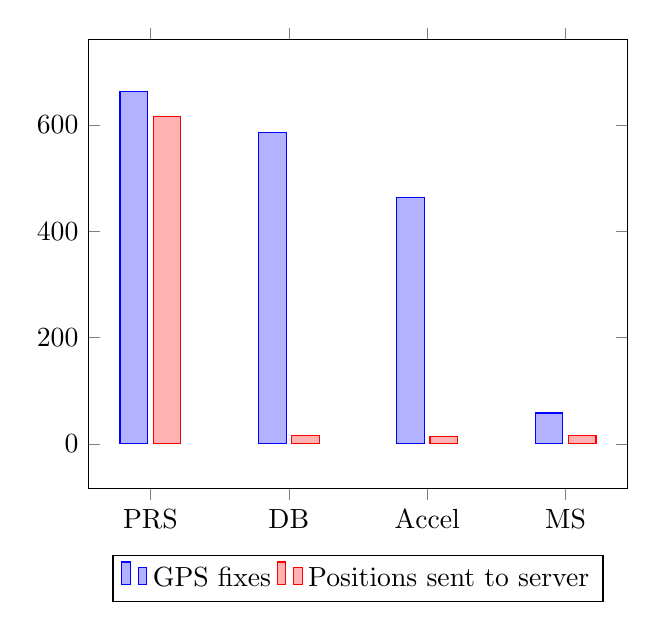
\begin{tikzpicture}
\begin{axis}
	[ybar,
	enlargelimits=0.15,
	legend style={at={(0.5,-0.15)},	anchor=north,legend columns=-1},
	symbolic x coords={PRS, DB, Accel, MS},
	xtick=data]
	
\addplot coordinates
	{(PRS,663) (DB,585) (Accel,463) (MS,58)};
\addplot coordinates
	{(PRS,616) (DB,15) (Accel,14) (MS,16)};

\legend{GPS fixes, Positions sent to server}
\end{axis}
\end{tikzpicture}
\label{locationsreadandsent}
\caption{Comparison of the amount of GPS fixes read and the amount of fixes sent to the server.}
\end{figure}

As seen in figure-\ref{locationsreadandsent} the three distance based algorithms lower the amount of readings sent a lot compared to the periodic strategy. Thus these looses some of the accuracy, but with the benefit of reading and sending less data. Most notably the distance based with the accelerometer and the max speed reads fewer data while offline too. The max speed algorithm also have a way lower accuracy, but would be optimal for cases where only a rough position is needed. On the other hand if accuracy is needed the accelerometer seems to be a good tradeoff.

Mostly the walking paths (shown in the appendix) is quite close to the ground truth, but for the distance based algorithms the corners can be cut off.

\begin{figure}[h]
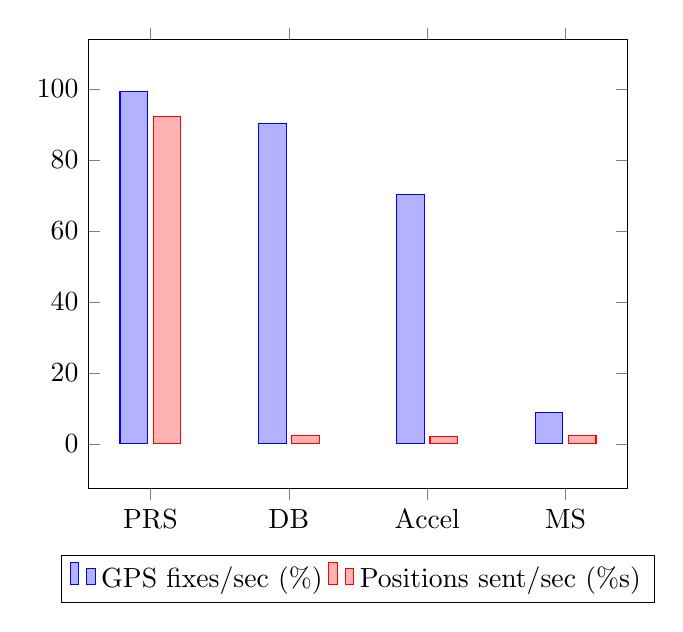
\begin{tikzpicture}
\begin{axis}
	[ybar,
	enlargelimits=0.15,
	legend style={at={(0.5,-0.15)},	anchor=north,legend columns=-1},
	symbolic x coords={PRS, DB, Accel, MS},
	xtick=data]
	
\addplot coordinates
	{(PRS,99.25) (DB,90.28) (Accel,70.15) (MS,8.92)};
\addplot coordinates
	{(PRS,92.22) (DB,2.31) (Accel,2.12) (MS,2.46)};

\legend{GPS fixes/sec (\%), Positions sent/sec (\%s)}
\end{axis}
\end{tikzpicture}
\caption{The amount of fixes read and the amount of positions sent to the server relative to time.}
\label{fixesandsendrelativetotime}
\end{figure}

\section{Conclusion}
It is possible to reduce both the number of GPS fixes and the number of connections to servers, and still track the target. However the use case must be taking into account, due the different limitations of the algorithms. Depending on the use case the distance based with max speed (DBRS -MS) and accelerometer (DBRS - A) seems to perform quite well. The DBRS - MS does very few readings at the cost of accuracy, whereas DBRS -A gives very accurate locations, but also used a lot more readings. The DBRS - MS could be improved to gain further accuracy, but this would also increase the amount of readings. It also seems that a the alsorithms has weaknesses when the target does not walk in straight paths. But with these algorithms the battery consumption can be reduced and devices can use pervasive positioning for longer time.

\end{document}
